\chapter{تنظيم الأجهزة العصبية}\label{ch:b3:nervous-systems}

لقنديل البحر بضعة آلاف من العصبونات في شبكة بلا مركز، وهو
يسبح ويأكل ويعدّل وضعه. وللأخطبوط نصف مليار، ثلثاها في
أذرعه، وكل ذراع تقدر على حل مشكلة لم يُخبَر الدماغ بها. ولك
أنت ستة وثمانون مليارًا، توصلها مئة تريليون مشبك، وتعمل على
عشرين واطًا --- أي خُمس طاقتك مقابل اثنين في المئة من كتلتك
--- وقد رأى سانتياغو رامون إي كاخال، وهو يرسمها خلية خلية
في تسعينيات القرن التاسع عشر من شرائح مصبوغة بالفضة، أنها
خلايا منفصلة تتلامس من غير أن تندمج وأن الإشارات تجري فيها
في اتجاه واحد. وقد تناول المجلد السابق العصبون: كمونه
الساكن، وكمون عمله، ومشبكه. ويتناول هذا الفصل ما تُوصَل
إليه العصبونات: الكبل المنفعل الذي يحد مدى انتشار الإشارة
وسرعتها، والدارات --- المنعكس، والمذبذب، والتثبيط المحيط
--- التي يُركَّب منها السلوك، وخطة الجهاز العصبي في
الفقاريات وخطة الدبقيات التي تبقيه عاملًا، وميزانيته
الطاقية، والطرق التي وزّعت بها حيوانات مختلفة عصبوناتها.

\section{العصبونات والدبقيات}

\begin{definition}[خلايا الجهاز العصبي]\label{def:b3:nervous-systems:cells}
\index{عصبون!الأنماط}\index{دبق}\index{خلية نجمية}\index{قليلة التغصن}\index{مييلين}\index{دبقية صغيرة}\index{عصبون بيني}
تأتي العصبونات في بضع معماريات تتكرر في أنحاء الدماغ:
الخلايا \emph{الهرمية}، وهي العصبونات الإسقاطية المهيِّجة في
القشرة، لها تغصن قمّي طويل ومحوار قد يمتد مترًا؛ وخلايا
\emph{بركنجي} في \omterm{def:b3:nervous-systems:plan}{المخيخ}، وشجرتها التغصنية المسطحة تتلقى
مئتي ألف مشبك؛ والعصبونات الحسية ذات استطالة إلى المحيط
وأخرى إلى النخاع؛ و\emph{العصبونات البينية}، وهي خلايا قصيرة
المحوار تبقى داخل منطقة واحدة، ومعظمها مثبِّط. ونحو أربعة من
كل خمسة عصبونات قشرية تطلق الغلوتامات وتهيّج؛ وواحد من كل
خمسة يطلق GABA ويثبّط. وأما \emph{الدبقيات}، وهي بعدد
العصبونات، فتفعل الباقي. و\emph{الخلايا النجمية} تلف المشابك
والأوعية الدموية: فهي تلتقط البوتاسيوم الذي تطلقه العصبونات
المشتعلة والغلوتامات التي تسكبها المشابك، وتوفر اللاكتات،
وتنظم الجريان الدموي موضعيًا، وتستحث \omterm{prop:b3:nervous-systems:barrier-budget}{الحاجز الدموي الدماغي}
وتصونه. و\emph{قليلات التغصن} في الجهاز العصبي المركزي
و\emph{خلايا شوان} في المحيط تلف المحاوير في \emph{مييلين}،
وهو عشرات الطبقات من الغشاء تعزل المحوار بين العُقد التي
تجلس فيها القنوات. و\emph{الدبقيات الصغيرة} هي بلعميات
الدماغ المقيمة، تقلّم المشابك في النماء وتصفّي الحطام.
وتبطّن الخلايا البِطانية البُطينات وتصنع \omterm{prop:b3:nervous-systems:barrier-budget}{السائل الدماغي
الشوكي}.
\end{definition}

\begin{proof}[شواهد]
صبغة كرومات الفضة عند غولجي (1873) سوّدت، لأسباب مجهولة،
نحو عصبون من كل مئة، تسويدًا كاملًا، وتركت الباقي غير مرئي
--- فأمكن أن تُرى خلية واحدة كاملة في تشابك الملايين. وقرأ
غولجي مستحضراته هو شبكةً متصلة؛ وأما كاخال، منذ 1888،
مستعملًا الصبغة نفسها على نسيج جنيني تكون الخلايا فيه أبسط،
فرأى أن كل خلية تنتهي حرة، وأن التغصنات تختلف عن المحوار،
وأن المحاوير تنتهي على تغصنات خلايا أخرى وأجسامها من غير أن
تتصل بها. ومن ترتيب الخلايا الحسية والحركية استنتج اتجاه
الجريان --- من التغصن إلى الجسم إلى المحوار --- وهو
\emph{قانون الاستقطاب الحركي}. وسمّى شيرينغتون الفجوة
\emph{المشبك} عام 1897؛ وأظهره المجهر الإلكتروني عام 1954.
\end{proof}

\begin{omfigure}
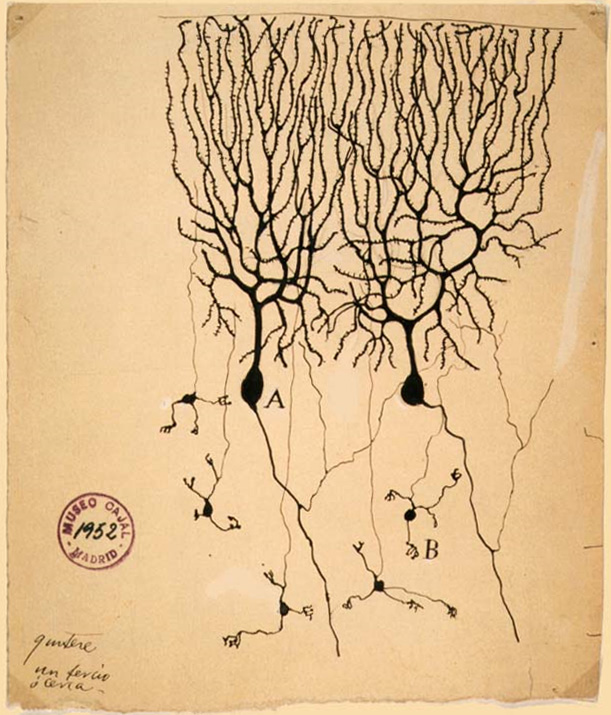
\includegraphics[width=0.30\linewidth]{images/book5/cajal-purkinje.jpg}\hspace{0.04\linewidth}
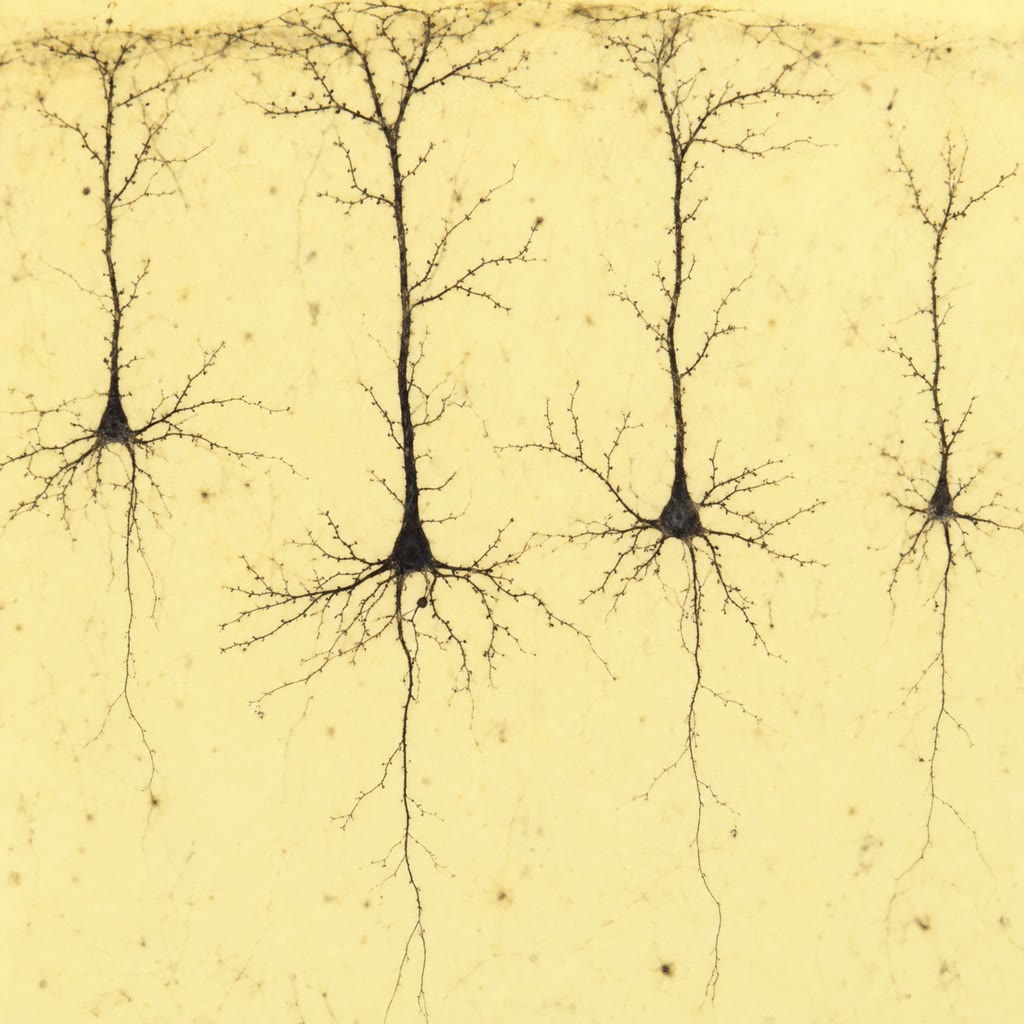
\includegraphics[width=0.30\linewidth]{images/book5/ai/b5-17-cortex-neurons.jpg}\hspace{0.04\linewidth}
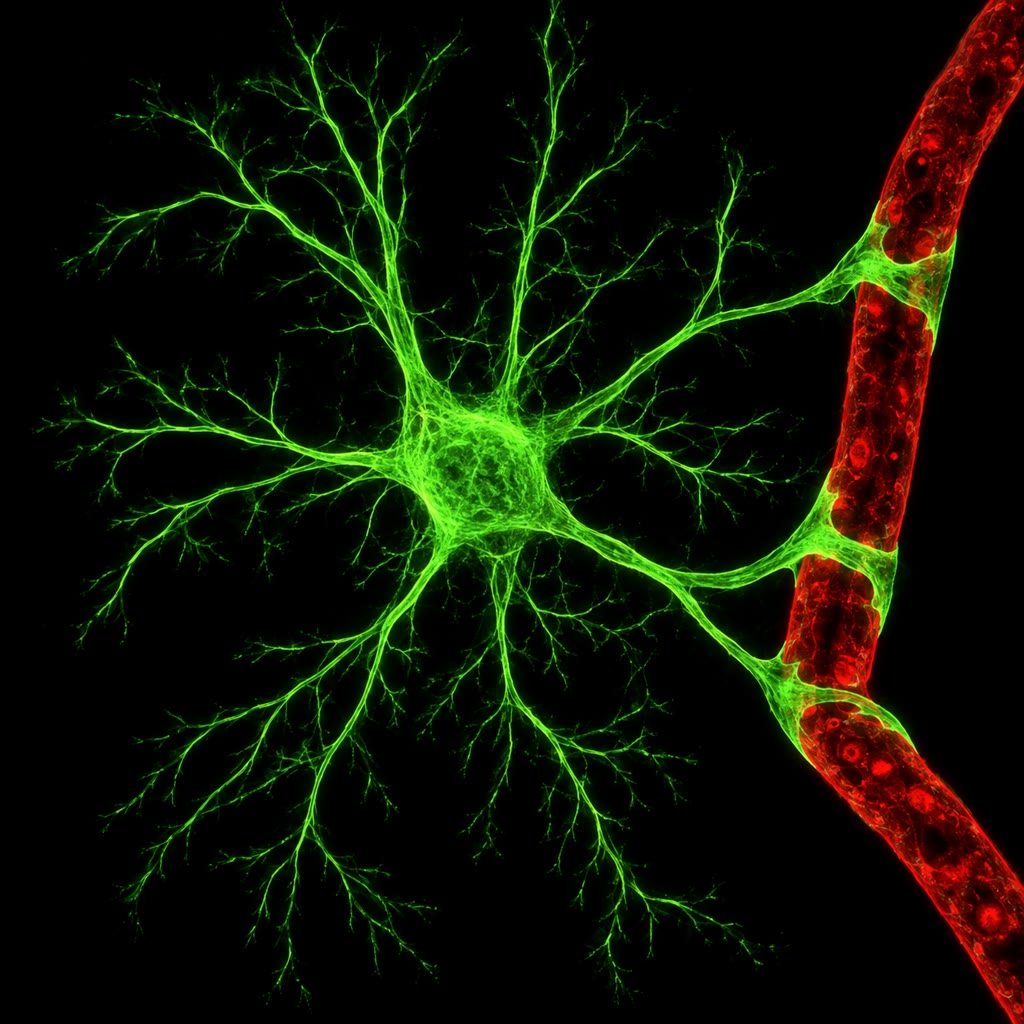
\includegraphics[width=0.30\linewidth]{images/book5/ai/b5-17-astrocyte.jpg}

{\small يسارًا: خلية بركنجي من \omterm{def:b3:nervous-systems:plan}{المخيخ} رسمها كاخال (1899) من
مقطع مصبوغ بصبغة غولجي --- الشجرة التغصنية كلها لخلية
واحدة، وهي الحجة على أن العصبون وحدة (ملكية عامة). وفي
الوسط: عصبونات هرمية من القشرة في صبغة غولجي. ويمينًا: \omterm{def:b3:nervous-systems:cells}{خلية
نجمية} (بالأخضر) وأقدامها الطرفية على شعيرة (بالأحمر).}
\end{omfigure}

\section{العصبون كبلًا}

\begin{theorem}[معادلة الكبل في الحالة المستقرة]\label{thm:b3:nervous-systems:cable}
\index{معادلة الكبل}\index{ثابت الطول}\index{ثابت الزمن!الغشاء}\index{سرعة النقل}
نمذج تغصنًا أو محوارًا غير مُميَلن أسطوانةً قطرها $d$
مقاومية عصارتها $R_{i}$ ومقاومة غشائها النوعية $R_{m}$
(مقاومة في مساحة) وسعته $C_{m}$ في وحدة المساحة. فتكون
المقاومة المحورية في وحدة الطول $r_{i} = 4R_{i}/\pi d^{2}$
ومقاومة الغشاء $r_{m} = R_{m}/\pi d$. وينتشر جهد ثابت
$V_{0}$ مطبَّق عند $x = 0$ على امتداد الليف على الصورة
\[
V(x) = V_{0}\,e^{-x/\lambda}, \qquad
\lambda = \sqrt{\frac{r_{m}}{r_{i}}} = \sqrt{\frac{R_{m}\,d}{4R_{i}}},
\]
حيث $\lambda$ هو \emph{\omterm{thm:b3:nervous-systems:cable}{ثابت الطول}}: أي المسافة التي تهبط
عليها إشارة منفعلة إلى $1/e$، وهو ينمو مع الجذر التربيعي
للقطر. ويُشحن الغشاء عند \emph{ثابت الزمن} $\tau =
R_{m}C_{m}$، وهو مستقل عن الهندسة. وكمون العمل، الذي يجدّد
نفسه، يسير على امتداد محوار غير مُميَلن بسرعة تتناسب مع
$\lambda/\tau$ ومن ثم مع $\sqrt{d}$؛ وعلى امتداد محوار
مُميَلن، حيث يقفز من عقدة إلى عقدة، بسرعة تتناسب مع $d$ ---
أي نحو \qty{6}{m/s} لكل ميكرومتر من القطر.
\end{theorem}
\begin{proof}
ليكن $I(x)$ التيار المحوري. فقانون أوم على امتداد اللبّ
يعطي $\mathrm{d}V/\mathrm{d}x = -r_{i}I$؛ وحفظ الشحنة في
الحالة المستقرة يقول إن التيار المحوري المفقود بين $x$
و$x + \mathrm{d}x$ يتسرب عبر الغشاء، أي
$\mathrm{d}I/\mathrm{d}x = -V/r_{m}$. وباشتقاق الأولى
وتعويض الثانية نجد
$\mathrm{d}^{2}V/\mathrm{d}x^{2} = (r_{i}/r_{m})V = V/\lambda^{2}$، وهي
معادلة خطية من الرتبة الثانية حلها المحدود عند $x \to \infty$ هو
$V_{0}e^{-x/\lambda}$. وبتعويض $r_{m} = R_{m}/\pi d$ و$r_{i} =
4R_{i}/\pi d^{2}$ نجد $\lambda^{2} = R_{m}d/4R_{i}$. وثابت الزمن
هو ثابت مقاومة وسعة على التوازي، $r_{m}c_{m} =
(R_{m}/\pi d)(C_{m}\pi d) = R_{m}C_{m}$. وأما السرعات: فالموجة
المجدِّدة لنفسها يجب أن تشحن الغشاء مسافة ثابت طول أمامها
في نحو ثابت زمن، فيكون $v \sim \lambda/\tau \propto \sqrt{d}$؛
وبين عُقد محوار مُميَلن يكون لغشاء ما بين العقدتين مقاومة
مرفوعة وسعة مخفوضة بفضل طبقات \omterm{def:b3:nervous-systems:cells}{المييلين} التي تزيد على المئة،
ويتناسب طول ما بين العقدتين مع $d$، فتكون النتيجة
$v \propto d$. وثوابت التناسب مُسلَّم بها.
\end{proof}

\begin{example}[أرقام لتغصن ولمحوارين]\label{ex:b3:nervous-systems:numbers}
تغصن قطره $d = \qty{2}{\micro m}$ عند $R_{m} = \qty{2e4}{\ohm.cm^2}$
و$R_{i} = \qty{100}{\ohm.cm}$: فيكون $\lambda = \sqrt{2\times 10^{4}\times
2\times 10^{-4}/400}\ \unit{cm} = \qty{0.1}{cm} = \qty{1}{mm}$ --- أي
إن كمونًا مشبكيًا في طرف تغصن طوله ميليمتر يبلغ جسم الخلية
بثلث حجمه، ولذلك تكون هندسة الشجرة التغصنية جزءًا من
حسابها. و$\tau = 2\times 10^{4}\times
10^{-6}\,\unit{F/cm^2}\cdot\unit{\ohm.cm^2} = \qty{20}{ms}$، وهي النافذة
التي يجب أن تصل الدخلات ضمنها لتتجامع. والمحوار العملاق
للحبّار، وقطره \qty{500}{\micro m}، غير مُميَلن، ينقل بنحو
\qty{25}{m/s}؛ وليفعل فقاري الشيء نفسه يستعمل محوارًا
مُميَلنًا قطره \qty{4}{\micro m}، أصغر منه مقطعًا بخمسة عشر
ألف ضعف --- وذلك سبب قدرة عصب فقاري على حمل عشرة آلاف ليف
سريع في حيز محوار حبّار واحد. ومحوار حركي قطره
\qty{20}{\micro m} ينقل بسرعة \qty{120}{m/s}؛ وحين يجرّد
التصلب المتعدد مييلينه تهبط السرعة عشرة أضعاف وقد يخفق
النقل كليًا عند الامتدادات العارية.
\end{example}

\begin{omfigure}
\begin{tikzpicture}
\begin{axis}[
  width=6.4cm, height=5.2cm,
  axis x line=bottom, axis y line=left,
  xmin=0, xmax=3, ymin=0, ymax=1.05,
  xlabel={المسافة (mm)}, ylabel={$V/V_{0}$},
  xlabel style={font=\small, at={(axis description cs:0.5,-0.12)}, anchor=north}, ylabel style={font=\small},
  tick label style={font=\scriptsize}, xtick={0,1,2,3}, ytick={0,0.37,1}, yticklabels={0,$1/e$,1},
  clip=false,
]
\addplot[very thick, omDef, domain=0:3, samples=60] {exp(-x/1.0)};
\addplot[very thick, omThm, domain=0:3, samples=60] {exp(-x/0.5)};
\node[font=\scriptsize, omDef, anchor=south west] at (axis cs:1.2,0.45) {$d = \qty{2}{\micro m}$، $\lambda = \qty{1}{mm}$};
\node[font=\scriptsize, omThm, anchor=north west] at (axis cs:0.8,0.22) {$d = \qty{0.5}{\micro m}$، $\lambda = \qty{0.5}{mm}$};
\end{axis}
\begin{axis}[
  at={(7.6cm,0)}, anchor=south west,
  width=6.4cm, height=5.2cm,
  xmode=log, ymode=log,
  xmin=0.1, xmax=1000, ymin=0.1, ymax=200,
  xlabel={قطر المحوار ($\unit{\micro m}$)}, ylabel={السرعة (m/s)},
  xlabel style={font=\small, at={(axis description cs:0.5,-0.12)}, anchor=north}, ylabel style={font=\small},
  tick label style={font=\scriptsize},
  clip=false,
]
\addplot[very thick, omDef, domain=1:25, samples=2] {6*x};
\addplot[very thick, omThm, domain=0.2:1000, samples=2] {1.1*sqrt(x)};
\fill[omThm] (axis cs:500,25) circle (2pt); \node[font=\scriptsize, anchor=north east] at (axis cs:500,23) {محوار الحبّار العملاق};
\fill[omDef] (axis cs:20,120) circle (2pt); \node[font=\scriptsize, anchor=west] at (axis cs:26,120) {محوار حركي بشري};
\node[font=\scriptsize, omDef, anchor=north west, align=left] at (axis cs:1.2,60) {مُميَلن: $v \propto d$};
\node[font=\scriptsize, omThm, anchor=north west, align=left] at (axis cs:2,0.7) {غير مُميَلن: $v \propto \sqrt{d}$};
\end{axis}
\end{tikzpicture}

{\small يسارًا: الهبوط المنفعل لإشارة ثابتة على امتداد تغصن،
عند قطرين --- \omterm{thm:b3:nervous-systems:cable}{وثابت الطول} ينمو مع $\sqrt{d}$. ويمينًا: \omterm{thm:b3:nervous-systems:cable}{سرعة
النقل} في مقابل القطر؛ \omterm{def:b3:nervous-systems:cells}{والمييلين} يجعل ليفًا قطره
\qty{4}{\micro m} يفعل ما يحتاج محوار غير مُميَلن إلى نصف
ميليمتر ليفعله.}
\end{omfigure}

\section{الدارات}

\begin{definition}[الدارات الأولية]\label{def:b3:nervous-systems:circuits}
\index{قوس منعكس}\index{تثبيط متبادل}\index{تثبيط أمامي}\index{تثبيط راجع}\index{تقارب}\index{تشعّب}
\emph{قوس المنعكس} أقصر طريق من مستقبِل إلى مستجيب: ففي
منعكس الركبة، يدخل وارد من مغزل عضلي إلى النخاع ويتشابك
مباشرةً على العصبونات الحركية للعضلة نفسها، فتقبضها بعد
الطرقة بنحو \qty{30}{ms} --- مشبك واحد، بلا دماغ. والوارد
نفسه يهيّج عصبونًا بينيًا مثبِّطًا للعصبونات الحركية للعضلة
المضادة (\emph{التثبيط المتبادل})، حتى لا تقاوم القابضةُ
انقباضَ الباسطة. ومعظم الدارات مبني من بضع نُمَيطات:
\emph{التشعّب}، أي عصبون واحد يسوق كثيرين، و\emph{التقارب}،
أي كثيرون على واحد، وهو يجمع الأدلة؛ و\emph{التثبيط
الأمامي}، إذ يهيّج دخلٌ هدفًا وعصبونًا بينيًا يثبّط الهدف
بعد ميلي ثانية، فيحدّ الاستجابة زمنيًا؛ و\emph{التثبيط
الراجع}، إذ يهيّج خرج الهدف نفسه عصبونًا بينيًا يثبّطه،
فيحد الاشتعال، وينتج، إذا امتد إلى الجيران، التثبيط الجانبي
الذي يحدّ التباين (\cref{ch:b3:sensory-systems})؛ و\emph{رفع
التثبيط}، أي تثبيط مثبِّط، وهي طريقة العقد القاعدية في إطلاق
حركة.
\end{definition}

\begin{omfigure}
\begin{tikzpicture}[every node/.style={font=\scriptsize}, >=stealth]
  % spinal cord cross-section (schematic)
  \draw[thick, omDef!60, fill=omDef!8] (5.4,1.5) ellipse (2.0 and 1.5);
  \draw[thick, gray, fill=gray!15] (5.4,1.5) .. controls (4.7,2.4) and (4.0,2.6) .. (4.0,1.9) .. controls (4.0,1.2) and (4.6,0.9) .. (4.8,0.5) .. controls (5.0,0.2) and (5.8,0.2) .. (6.0,0.5) .. controls (6.2,0.9) and (6.8,1.2) .. (6.8,1.9) .. controls (6.8,2.6) and (6.1,2.4) .. (5.4,1.5);
  \node[above] at (5.4,3.05) {النخاع الشوكي};
  % muscles
  \draw[thick, omMeth!70!black, fill=omMeth!20] (0.2,0.2) rectangle (1.4,2.0); \node[below, align=center] at (0.8,0.1) {باسطة\\(رباعية الرؤوس)};
  \draw[thick, omThm!70!black, fill=omThm!15] (0.2,-2.6) rectangle (1.4,-1.4); \node[below, align=center] at (0.8,-2.7) {قابضة\\(أوتار المأبض)};
  \fill[omProp] (0.8,1.3) ellipse (0.12 and 0.3); \node[left, font=\tiny] at (0.65,1.3) {مغزل};
  % Ia afferent to cord (dorsal)
  \draw[very thick, omProp] (0.9,1.3) .. controls (2.0,2.6) and (3.6,2.9) .. (4.8,2.2); \fill[omProp] (4.8,2.2) circle (0.09);
  \node[above, omProp] at (2.6,2.85) {وارد Ia: تمطط};
  % motor neuron to extensor
  \fill[omMeth!70!black] (5.0,0.9) circle (0.16);
  \draw[->, very thick, omMeth!70!black] (4.9,0.85) .. controls (3.4,0.3) and (2.0,0.4) .. (1.4,1.0);
  \draw[->, thick, omProp] (4.8,2.2) -- (5.0,1.1);
  % inhibitory interneuron to flexor motor neuron
  \fill[omThm] (6.1,1.7) circle (0.13);
  \draw[->, thick, omProp] (4.9,2.25) -- (6.0,1.8);
  \fill[omThm!70!black] (6.0,0.6) circle (0.16);
  \draw[-|, thick, omThm] (6.1,1.55) -- (6.0,0.8);
  \draw[->, very thick, omThm!70!black, dashed] (5.9,0.5) .. controls (4.8,-0.8) and (3.0,-1.6) .. (1.4,-2.0);
  % right-hand labels with leaders
  \node[right, omThm, font=\tiny] at (7.6,1.9) {عصبون Ia بيني مثبِّط}; \draw[gray, thin] (7.55,1.9) -- (6.25,1.7);
  \node[right, omMeth!70!black, font=\tiny, align=left] at (7.6,1.1) {عصبون الباسطة الحركي: مهيَّج}; \draw[gray, thin] (7.55,1.1) -- (5.15,0.9);
  \node[right, omThm!70!black, font=\tiny, align=left] at (7.6,0.3) {عصبون القابضة الحركي: مثبَّط}; \draw[gray, thin] (7.55,0.3) -- (6.15,0.6);
  \node[below] at (4.6,-0.15) {منعكس أحادي المشبك: $\sim$\qty{30}{ms}};
  \node[below, align=center] at (4.2,-2.0) {تثبيط متبادل:\\العضلة المضادة تسترخي};
\end{tikzpicture}

{\small منعكس التمطط. طرقة تمطّط مغازل الباسطة؛ فيهيّج وارد
Ia عصبونات الباسطة الحركية مباشرةً (مشبك واحد)، ويُسكت، عبر
\omterm{def:b3:nervous-systems:cells}{عصبون بيني} مثبِّط، عصبونات القابضة.}
\end{omfigure}

\begin{proposition}[المولّدات النمطية المركزية]\label{prop:b3:nervous-systems:cpg}
\index{مولّد نمطي مركزي}\index{مذبذب نصفي المركز}
الحركات الإيقاعية --- التنفس، والمشي، والسباحة، والمضغ ---
تنتجها دارات في \omterm{def:b3:nervous-systems:plan}{جذع الدماغ} \omterm{def:b3:nervous-systems:plan}{والنخاع الشوكي} تتذبذب من تلقاء
نفسها، وهي \emph{المولّدات النمطية المركزية}، التي تعدّلها
التغذية الراجعة الحسية ولا تصنعها: فنخاع قط مقطوع عن الدماغ
ومحروم من أعصابه الحسية لا يزال ينتج نمط الخطو المتناوب.
وأبسط تصميم هو \emph{نصف المركز} عند براون (1911): مجموعتان
من العصبونات تثبّط كل منهما الأخرى. فأيتهما اشتعلت أسكتت
شريكتها؛ غير أن المجموعة المشتعلة تتعب --- إذ تُعطَّل
قنواتها، ويضعف تثبيطها لشريكتها --- فتشتعل الشريكة، وقد
تحررت، وتُسكت الأولى بدورها: فيكون التناوب، بدور يحدده ثابت
زمن التعب لا أي ساعة. والإيقاع التنفسي ينشأ في عنقود من بضعة
آلاف من العصبونات في البصلة (معقد ما قبل بوتزنغر)، يشتعل
دفقات من الولادة إلى الموت؛ وسباحة الجلكى سلسلة من أنصاف
المراكز على امتداد نخاعها، كل واحد متأخر عن سابقه فتسير
موجة نحو الذنب.
\end{proposition}

\begin{omfigure}
\begin{tikzpicture}[every node/.style={font=\scriptsize}, >=stealth]
  % half-centre
  \begin{scope}
    \draw[thick, fill=omDef!25] (0,0) circle (0.5); \node at (0,0) {L};
    \draw[thick, fill=omThm!25] (3,0) circle (0.5); \node at (3,0) {R};
    \draw[-|, very thick] (0.5,0.2) -- (2.5,0.2); \draw[-|, very thick] (2.5,-0.2) -- (0.5,-0.2);
    \node[above] at (1.5,0.3) {تثبيط متبادل};
    \draw[->, thick, omDef] (0,-0.5) -- (0,-1.3) node[below] {عضلات اليسار};
    \draw[->, thick, omThm] (3,-0.5) -- (3,-1.3) node[below] {عضلات اليمين};
    \draw[->, thick, gray] (-1.2,0.6) -- (-0.45,0.25) node[pos=0, above, align=center] {دفع مقوَّى\\من جذع الدماغ};
    \draw[->, thick, gray] (4.5,0.6) -- (3.45,0.25);
  \end{scope}
  % traces
  \begin{scope}[xshift=6.0cm, yshift=0.9cm]
    \node[left, omDef] at (0,0) {L};
    \foreach \x in {0,2,4} { \foreach \s in {0.1,0.2,...,0.9} \draw[omDef] (\x+\s,-0.15) -- (\x+\s,0.15); }
    \node[left, omThm] at (0,-1.0) {R};
    \foreach \x in {1,3,5} { \foreach \s in {0.1,0.2,...,0.9} \draw[omThm] (\x+\s,-1.15) -- (\x+\s,-0.85); }
    \draw[->] (0,-1.6) -- (6.2,-1.6) node[right] {الزمن};
    \draw[<->] (0,-2.0) -- (2,-2.0) node[midway, below] {الدور: يحدده التعب};
  \end{scope}
\end{tikzpicture}

{\small \omterm{prop:b3:nervous-systems:cpg}{مذبذب نصفي المركز}. مجموعتان متثابطتان تحت دفع ثابت
تتناوبان: فالجانب النشط يتعب، ويضعف تثبيطه، فيفلت الجانب
الآخر ويتولى. ولا عصبون فيهما إيقاعي بذاته.}
\end{omfigure}

\begin{method}[تتبع دارة]\label{met:b3:nervous-systems:tracing}
\index{تتبع الدارات}\index{علم البصريات الوراثي}
لإثبات أن العصبون A يسوق العصبون B وأن السبيل مهم لسلوك ما:
(1) التشريح --- احقن واسمًا يسير على امتداد المحاوير
(صباغًا، أو \omterm{def:b3:virology:virus}{فيروس} كلَب معدَّلًا يعبر مشبكًا واحدًا إلى
الوراء) وجِد الخلايا الموصولة؛ (2) الفيزيولوجيا --- سجّل من
B أثناء تنبيه A، وقس الكمون (الوصلة الأحادية المشبك تعطي
تأخيرًا ثابتًا قدره نحو ميلي ثانية) والإشارة (تهييج أو
تثبيط)؛ (3) الضرورة --- أسكِت A، بآفة، أو بالتبريد، أو بأن
تعبّر فيه عن مضخة كلوريد يسوقها الضوء ثم تسلّط الضوء
(\emph{\omterm{met:b3:nervous-systems:tracing}{علم البصريات الوراثي}})، وانظر هل يخفق السلوك؛ (4)
الكفاية --- فعّل A وحده، بقناة كاتيونية يسوقها الضوء، وانظر
هل يظهر السلوك؛ (5) في حيوان سليم، صوّر نشاط الجمهرة كلها
بكاشف كالسيوم أثناء أداء السلوك. وتثبت الدارة حين تتفق
الخمسة؛ ومعظم الدارات المنشورة تتفق فيها اثنتان أو ثلاث.
\end{method}

\section{خطة الجهاز العصبي في الفقاريات}

\begin{definition}[القسمان المركزي والمحيطي]\label{def:b3:nervous-systems:plan}
\index{نخاع شوكي}\index{جذع الدماغ}\index{مخيخ}\index{مهاد}\index{وطاء}\index{قشرة مخية}\index{جهاز عصبي ذاتي}\index{جهاز عصبي معوي}
\emph{الجهاز العصبي المركزي} هو الدماغ والنخاع الشوكي؛
و\emph{المحيطي} كل ما سواهما. و\emph{النخاع الشوكي} يتلقى
المحاوير الحسية عبر جذوره الظهرية ويرسل المحاوير الحركية
عبر جذوره البطنية، ومادته الرمادية فراشة من أجسام الخلايا،
ومادته البيضاء السبل المُميَلنة الصاعدة والنازلة.
و\emph{جذع الدماغ} --- البصلة، والجسر، والدماغ المتوسط ---
يحوي أنوية الأعصاب القحفية والمراكز التي تبقي التنفس وسرعة
القلب وضغط الدم ماضية بلا تفكير؛ وموت جذع الدماغ موت.
و\emph{المخيخ}، وفيه عصبونات أكثر مما في سائر الدماغ، يضبط
توقيت الحركة وتناسقها ويتعلم من الخطأ. و\emph{المهاد} ينقل
كل حاسة إلا الشم إلى القشرة وينقل أجوبة القشرة راجعةً؛
و\emph{الوطاء} تحته يدير الاستتباب --- الحرارة، والجوع،
والعطش، والساعة، والمحاور الصماوية في
\cref{ch:b3:endocrinology}. و\emph{العقد القاعدية} تنتقي بين
الأفعال الممكنة؛ و\emph{الحُصين} يصنع الذكريات
(\cref{ch:b3:learning-memory})؛ و\emph{القشرة المخية}، وهي
صفيحة من ست طبقات من الخلايا سماكتها ميليمتران إلى أربعة
ومساحتها ربع متر مربع، مطوية لتتسع، تفعل الباقي، في مناطق
مرسومة لكل حاسة وحركة وفي مناطق ترابطية بينها. والقسم
\emph{الذاتي} من الجهاز المحيطي يدير الأعضاء: فالسلسلة
\emph{الودّية}، التي تطلق النورأدرينالين، تعبّئ (فيرتفع
القلب، وتهبط الأمعاء، وتتسع الحدقتان)؛ والأعصاب \emph{نظيرة
الودية}، التي تطلق الأسيتيل كولين، تحفظ وتهضم؛ والجهاز
العصبي \emph{المعوي}، وفيه نصف مليار عصبون في جدار الأمعاء،
يدير الهضم بنفسه.
\end{definition}

\begin{omfigure}
\begin{tikzpicture}[every node/.style={font=\scriptsize}, >=stealth]
  % sagittal brain schematic
  \draw[thick, omDef!70, fill=omDef!15] (0,2.0) .. controls (0,4.6) and (3.5,5.4) .. (6.0,4.4) .. controls (7.6,3.7) and (7.4,2.2) .. (6.2,1.9) .. controls (5.4,1.7) and (5.2,1.3) .. (4.4,1.6) .. controls (3.0,1.3) and (1.2,1.4) .. (0,2.0);
  \node[align=center] at (3.0,3.9) {القشرة المخية: ست طبقات،\\مناطق حسية وحركية وترابطية};
  % basal ganglia / hippocampus (deep)
  \draw[thick, omProp!70, fill=omProp!25] (3.2,2.6) ellipse (0.9 and 0.45); \node[font=\tiny] at (3.2,2.6) {العقد القاعدية};
  \draw[thick, omProp!70, fill=omProp!25] (5.2,2.45) ellipse (0.88 and 0.3); \node[font=\tiny] at (5.2,2.45) {الحُصين};
  % thalamus, hypothalamus
  \draw[thick, omMeth!70!black, fill=omMeth!25] (4.0,1.95) ellipse (0.7 and 0.3); \node[font=\tiny] at (4.0,1.95) {المهاد};
  \draw[thick, omMeth!70!black, fill=omMeth!40] (4.0,1.42) ellipse (0.78 and 0.22); \node[font=\tiny] at (4.0,1.42) {الوطاء};
  % cerebellum
  \draw[thick, omThm!70, fill=omThm!20] (6.6,1.2) ellipse (0.9 and 0.6); \node[font=\tiny] at (6.6,1.2) {المخيخ};
  % brainstem
  \draw[thick, gray!70, fill=gray!20] (4.7,1.2) -- (5.5,1.2) -- (5.9,-0.3) -- (5.1,-0.3) -- cycle; \node[font=\tiny, rotate=-75] at (5.3,0.45) {جذع الدماغ};
  % spinal cord
  \draw[thick, gray!70, fill=gray!20] (5.2,-0.3) rectangle (5.8,-1.6); \node[right, font=\tiny] at (5.85,-1.0) {النخاع الشوكي};
  % labels with leaders on the right
  \node[right, align=left] at (7.8,3.4) {المهاد: ناقل لكل حاسة\\إلا الشم؛ والوطاء:\\الاستتباب، والساعة، والمحاور الصماوية};
  \draw[gray] (7.75,3.3) -- (4.7,1.95);
  \node[right, align=left] at (7.8,1.9) {المخيخ: التوقيت والتناسق،\\والتعلم من الخطأ};
  \draw[gray] (7.75,1.8) -- (7.5,1.4);
  \node[right, align=left] at (7.8,0.4) {جذع الدماغ: التنفس، والقلب،\\والأعصاب القحفية (البصلة،\\والجسر، والدماغ المتوسط)};
  \draw[gray] (7.75,0.4) -- (5.9,0.4);
  \node[right, align=left] at (7.8,-1.0) {النخاع الشوكي: المنعكسات،\\والمولّدات النمطية، والسبل صعودًا ونزولًا};
\end{tikzpicture}

{\small دماغ الفقاري في منظر سهمي، تخطيطيًا: القشرة فوق
الأنوية العميقة، \omterm{def:b3:nervous-systems:plan}{والمهاد} \omterm{def:b3:nervous-systems:plan}{والوطاء} في المركز، \omterm{def:b3:nervous-systems:plan}{والمخيخ} خلفًا،
\omterm{def:b3:nervous-systems:plan}{وجذع الدماغ} ممتدًا إلى النخاع.}
\end{omfigure}

\begin{proposition}[الحاجز الدموي الدماغي وميزانية الدماغ]\label{prop:b3:nervous-systems:barrier-budget}
\index{حاجز دموي دماغي}\index{سائل دماغي شوكي}\index{ميزانية الدماغ الطاقية}
شعيرات الدماغ مختومة بوصلات محكمة بين خلايا بطانتها، ملفوفة
بأقدام الخلايا النجمية، مزوّدة بناقلات تُدخل الغلوكوز
والأحماض الأمينية وتضخ كثيرًا مما سواها إلى الخارج: وذلك
\emph{\omterm{prop:b3:nervous-systems:barrier-budget}{الحاجز الدموي الدماغي}}، الذي يبقي التركيب الأيوني
للسائل خارج الخلوي في الدماغ ثابتًا من أجل السلوك الكهربائي
للعصبونات، والذي يستبعد معظم الأدوية (\qty{98}{\%} من
الجزيئات الصغيرة، والأضداد كلها) --- وهي المشكلة المركزية في
علم الأدوية العصبي. ويطفو الدماغ في \qty{150}{mL} من
\emph{\omterm{prop:b3:nervous-systems:barrier-budget}{السائل الدماغي الشوكي}}، يُصنع بنصف ميليلتر في الدقيقة
ويتجدد أربع مرات في اليوم، فيوسّده ويحمل عنه الفضلات، ولا
سيما أثناء النوم. وكلفة الدماغ: نحو \qty{20}{W} في البالغ،
أي \qty{20}{\%} من استقلاب الراحة، جلّها غلوكوز يُحرق إلى
ATP، ومعظم ذلك ATP تنفقه مضخة الصوديوم في استعادة التدرجات
التي تستنفدها كمونات العمل والتيارات المشبكية. وعند
\qty{50}{kJ} لكل مول من ATP تكون \qty{20}{W} هي $4\times 10^{-4}$
مول من ATP في الثانية، أي $2.4\times 10^{20}$ جزيء؛ ومقسومةً على
$8.6\times 10^{10}$ عصبون تعطي نحو $3\times 10^{9}$ من ATP لكل
عصبون في الثانية. وكمون عمل قشري بتبعاته المشبكية يكلف من
رتبة $10^{9}$ من ATP، فتسمح الميزانية بمعدل اشتعال وسطي قدره
بضع شوكات في الثانية لكل عصبون --- والعصبونات القشرية تشتعل
فعلًا بذلك المعدل تقريبًا. فالدماغ مبني على حد طاقي صارم،
ولذلك تكون إشاراته متناثرة، ومحاويره رفيعة، ومعلوماته
مرمَّزة بشوكات قليلة في خلايا كثيرة.
\end{proposition}
\admitted

\section{الأجهزة العصبية عبر الحيوانات}

\begin{definition}[الشبكات العصبية، والعقد، والأدمغة]\label{def:b3:nervous-systems:comparative}
\index{شبكة عصبية}\index{عقدة عصبية}\index{تمركز رأسي}\index{تدمغن}
للاذعات (قنديل البحر، والهيدرا) \emph{شبكة عصبية}: عصبونات
موزعة في جدار الجسم، موصولة في كل اتجاه، مع تكاثفات حلقية
حول حافة الجرس تنسّق السباحة --- بلا مركز، والنقل في
الاتجاهين على امتداد كل خلية. والحيوانات ثنائية التناظر
تركّز العصبونات في \emph{عقد} --- عناقيد ذات نسيج عصبي مشترك
--- مرتبة على امتداد حبل بطني في المفصليات والحلقيات، مع
عقدة رأسية متضخمة حيث تكون أعضاء الحس: وذلك \emph{التمركز
الرأسي}. وتتباين الرخويات من العقد البسيطة في المَحار إلى
الأخطبوط، وعصبوناته البالغة نصف مليار هي أكثر ما لأي
لافقاري، وثلثاها في الأذرع، ويتحكم حبل كل ذراع بمدّها
وقبضها. وأما الفقاريات فتبني أنبوبًا ظهريًا أجوف، متوسعًا
في الأمام إلى الدماغ الذي في القسم السابق، محميًا بالعظم
وبحاجز، ومُميَلنًا. وجزيئات الإشارة نفسها، والقنوات،
والنواقل، وكثير من مورّثات النماء نفسها (شفرة Hox في الدماغ
الخلفي، وعوامل تنميط العين) تشغّلها جميعًا: فالأجزاء قديمة
مشتركة، والترتيبات متنوعة.
\end{definition}

\begin{example}[عدّ العصبونات]\label{ex:b3:nervous-systems:counts}
للخيطية $302$ عصبون، كل واحد مسمّى وكل مشبك مرسوم؛ ولذبابة
الفاكهة $1.4\times 10^{5}$؛ ولنحلة العسل $10^{6}$؛ وللفأر
$7\times 10^{7}$؛ وللأخطبوط $5\times 10^{8}$؛ وللإنسان $8.6\times
10^{10}$؛ وللفيل $2.6\times 10^{11}$، معظمها في مخيخه. وتتدرج
كتلة الدماغ مع كتلة الجسم في الثدييات تدرجًا يقارب
$M_{\text{brain}} \propto M_{\text{body}}^{0.75}$، فيكون دماغ
الفأر نسبةً من جسمه أكبر من نسبة دماغ الفيل من جسمه؛
والأنواع فوق الخط المناسب لحجمها --- الدلافين، والرئيسيات،
والإنسان بعامل سبعة --- يقال إنها متدمغنة. والذي يتابع
الإدراك أفضل متابعة ليس كتلة الدماغ بل عدد العصبونات في
\omterm{def:b3:nervous-systems:plan}{القشرة المخية}: نحو $1.6\times 10^{10}$ في الإنسان، و$5.6\times 10^{9}$
في الفيل ودماغه أكبر ثلاث مرات، و$2\times 10^{9}$ في
الشمبانزي. فدماغ الإنسان ليس خاصًا في خلاياه ولا في خطته؛
وإنما فيه من العصبونات القشرية أكثر مما في أي دماغ آخر،
مرصوصة أكثف، والعدد لا الوزن هو ما يبدو أنه يُحسب.
\end{example}

\begin{omfigure}
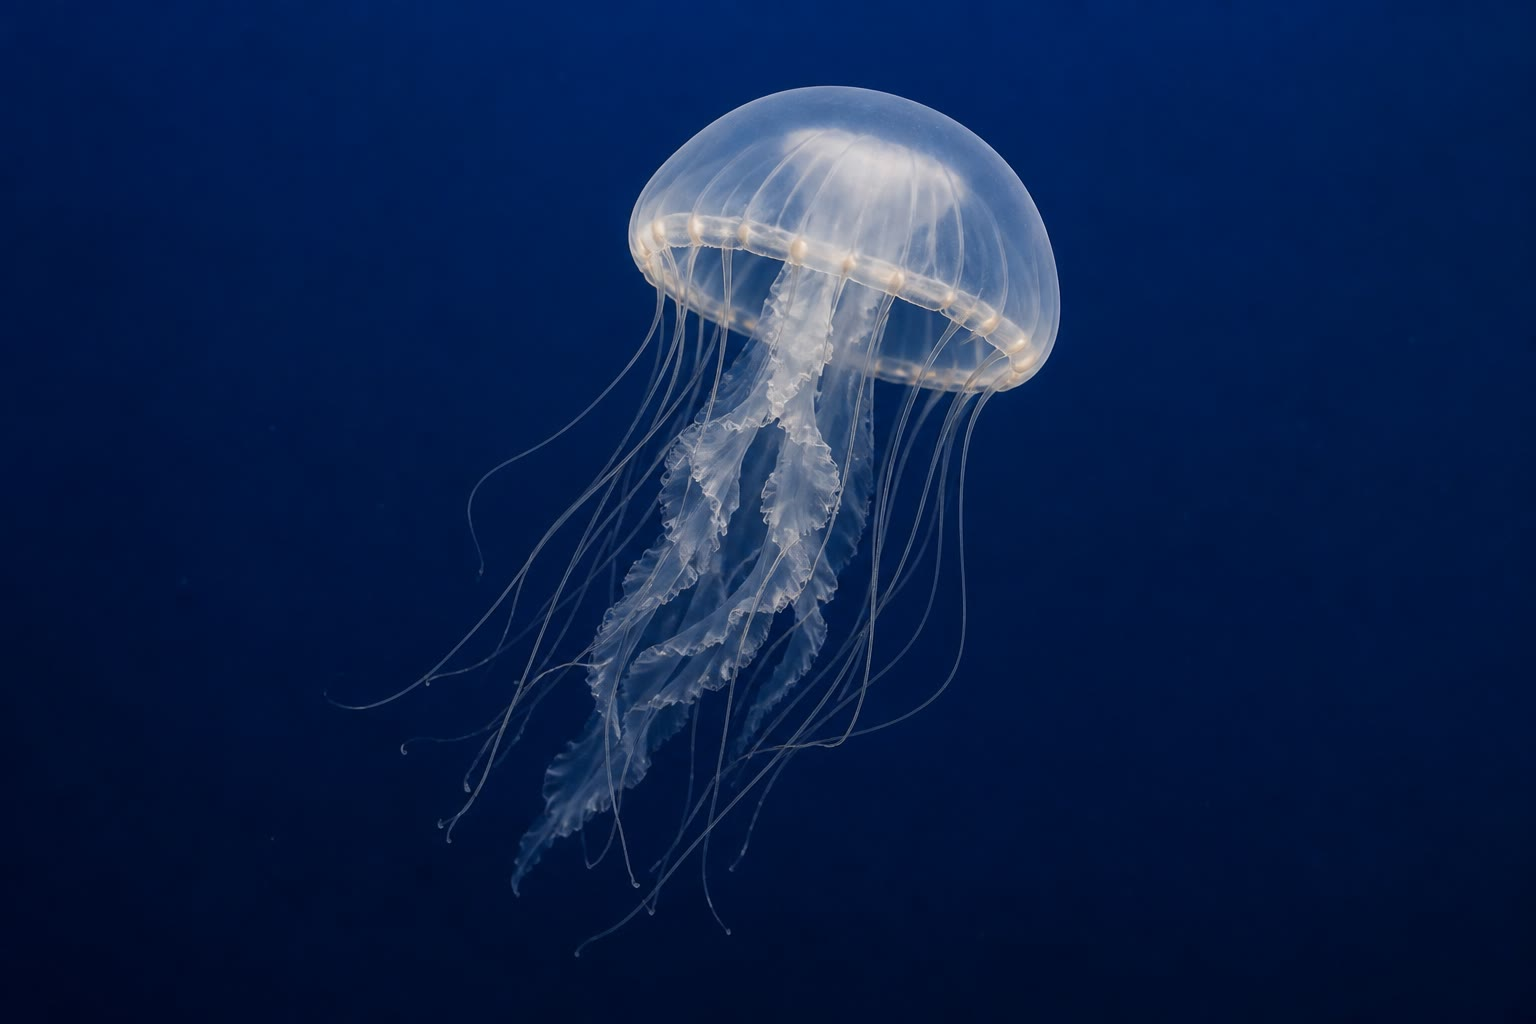
\includegraphics[width=0.46\linewidth]{images/book5/ai/b5-17-jellyfish.jpg}\hspace{0.04\linewidth}
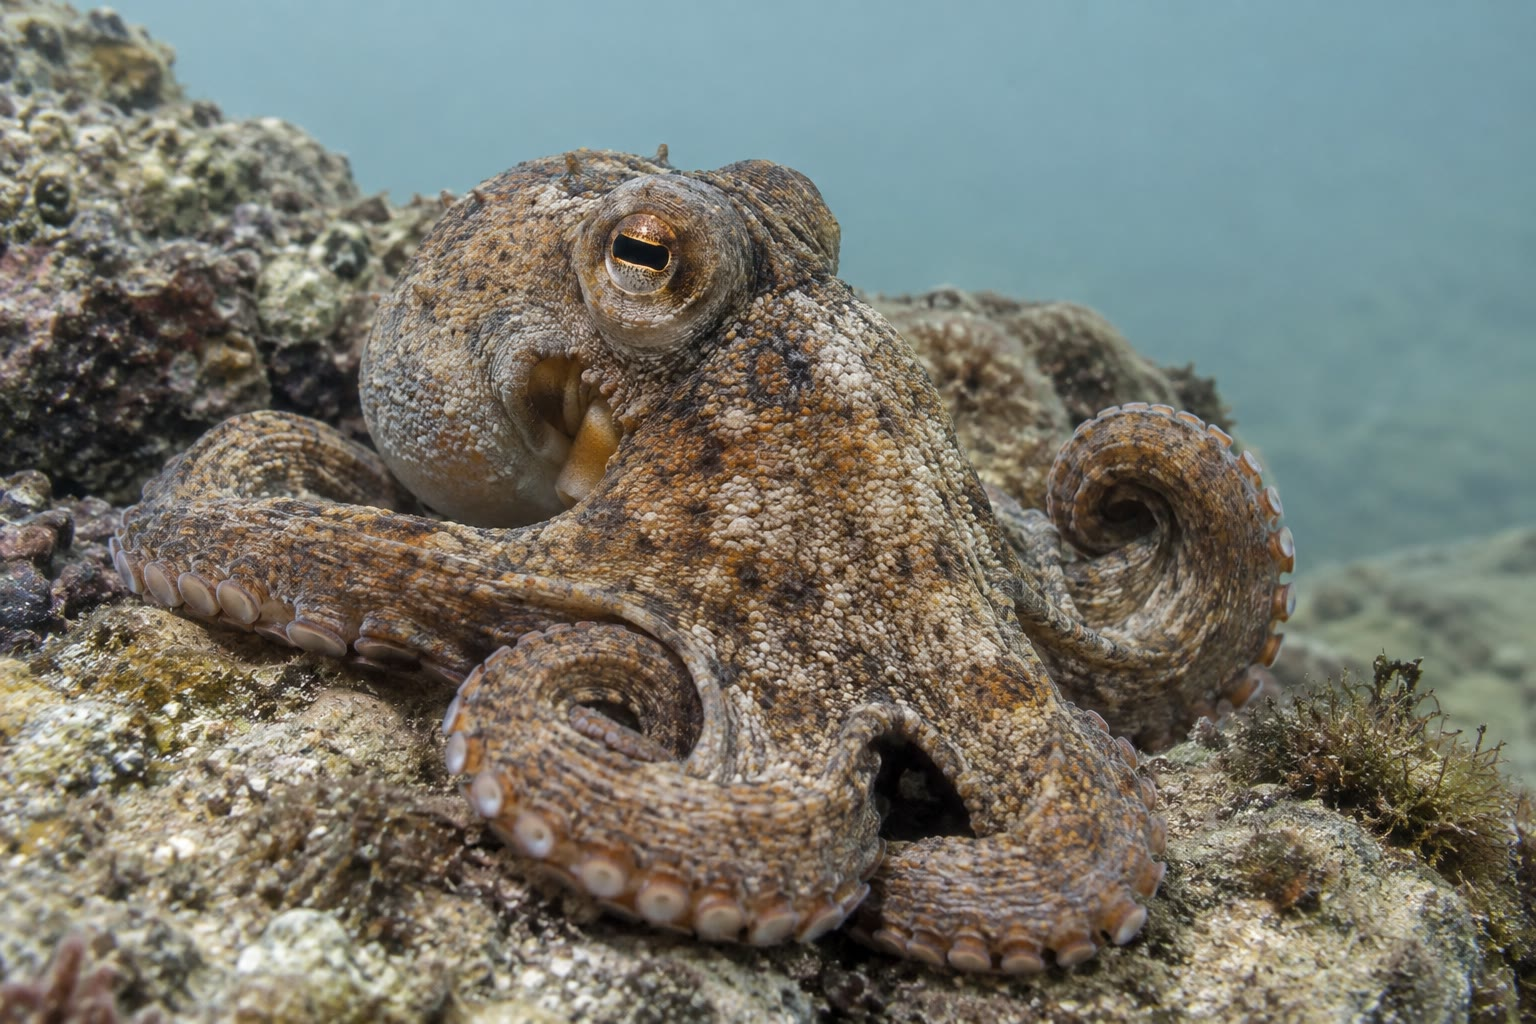
\includegraphics[width=0.46\linewidth]{images/book5/ai/b5-17-octopus.jpg}

{\small طريقتان في تنظيم العصبونات. يسارًا: قنديل بحر،
تنسّق شبكته العصبية وحلقاته الحافّية السباحة بلا دماغ.
ويمينًا: أخطبوط، له نصف مليار عصبون، معظمها في الأذرع، وأكبر
دماغ لأي لافقاري.}
\end{omfigure}

\begin{remark}[فيمَ الجهاز العصبي]\label{rem:b3:nervous-systems:for}
لا جهاز عصبي للنبات ولا للفطور ولا للإسفنجيات؛ والحيوان
الذي يتحرك يحتاج إلى واحد، وتفصيل الأجهزة العصبية يتابع
مطالب الحركة، والإحساس عن بُعد، والتنبؤ بما سيحدث تاليًا.
\omterm{thm:b3:nervous-systems:cable}{فمعادلة الكبل} تضع الفيزياء --- إلى أي بُعد وبأي سرعة تسير
إشارة عند قطر وعزل معينين؛ وميزانية الطاقة تضع الاقتصاد؛
وضمن هذين الحدين تنتج العصبونات نفسها، مرتبةً شبكات أو
عقدًا أو قشرة، نبضة قنديل بحر، أو تمويه أخطبوط، أو هذه
الجملة. ويتناول الفصلان التاليان طرف الدخل والتخزين: كيف
تحوّل الحواس العالم إلى شوكات، وكيف تتغير المشابك حتى
يُتذكَّر العالم بعد لقائه.
\end{remark}

\section{تمارين}

\begin{exercise}[$\star$]\label{exo:b3:nervous-systems:1}
سمّ أنماط الدبقيات الأربعة ووظيفة واحدة لكل نمط، وقل أيّ
اثنين يصنعان \omterm{def:b3:nervous-systems:cells}{المييلين} وأين.
\end{exercise}

\begin{exercise}[$\star$]\label{exo:b3:nervous-systems:2}
ماذا أتاحت صبغة غولجي، وماذا استنتج كاخال منها، وماذا استنتج
غولجي؟ وأيهما كان محقًا، وكيف حُسم الأمر؟
\end{exercise}

\begin{exercise}[$\star$]\label{exo:b3:nervous-systems:3}
صف \omterm{def:b3:nervous-systems:circuits}{قوس منعكس} الركبة واشرح لماذا يستغرق \qty{30}{ms} فقط
بينما تستغرق ركلة إرادية عشرة أضعاف ذلك.
\end{exercise}

\begin{exercise}[$\star$]\label{exo:b3:nervous-systems:4}
اذكر آثار الودي ونظير الودي على القلب، والحدقة، والأمعاء،
والطرق الهوائية، والناقل الذي يستعمله كل قسم عند الهدف.
\end{exercise}

\begin{exercise}[$\star\star$]\label{exo:b3:nervous-systems:5}
احسب \omterm{thm:b3:nervous-systems:cable}{ثابت الطول} لمحوار قطره \qty{1}{\micro m} عند $R_{m}
= \qty{1e4}{\ohm.cm^2}$ و$R_{i} = \qty{100}{\ohm.cm}$، ونسبة
ما يبقى من إشارة بعد \qty{2}{mm}. وأي قطر يضاعف $\lambda$؟
\end{exercise}

\begin{exercise}[$\star\star$]\label{exo:b3:nervous-systems:6}
محوار حسي قطره \qty{12}{\micro m} يمتد \qty{1.2}{m} من إصبع
القدم إلى النخاع، ومحوار حركي قطره \qty{15}{\micro m} يعود.
فمع \qty{6}{m/s} لكل ميكرومتر و\qty{0.5}{ms} لكل مشبك، قدّر
أدنى كمون لمنعكس سحب نخاعي فيه \omterm{def:b3:nervous-systems:cells}{عصبون بيني} واحد. وكم يستغرق
بمحاوير غير مميلنة بالقطر نفسه عند
$v = 1.1\sqrt{d}$؟
\end{exercise}

\begin{exercise}[$\star\star$]\label{exo:b3:nervous-systems:7}
مستعينًا بميزانية الدماغ من
\cref{prop:b3:nervous-systems:barrier-budget}، قدّر كم من ATP
يقدر عصبون على إنفاقه في الثانية، وإذا كانت الشوكة بمشابكها
تكلف $2\times 10^{9}$ من ATP، فما معدل الاشتعال الوسطي الذي
تسمح به الميزانية؟ وبماذا يتنبأ ذلك عن الترميز؟
\end{exercise}

\begin{exercise}[$\star\star$]\label{exo:b3:nervous-systems:8}
اشرح لماذا يحتاج \omterm{prop:b3:nervous-systems:cpg}{مذبذب نصفي المركز} إلى التعب (أو إلى عملية
بطيئة أخرى) ليتذبذب، وماذا سيحدث لعصبونين متثابطين لا
يتعبان أبدًا.
\end{exercise}

\begin{exercise}[$\star\star$]\label{exo:b3:nervous-systems:9}
يستبعد \omterm{prop:b3:nervous-systems:barrier-budget}{الحاجز الدموي الدماغي} الدوبامين الناتج من L-dopa
لكنه يُدخل L-dopa. اشرح كيف يُستغل ذلك في داء باركنسون
ولماذا يصعب إيصال الأضداد إلى بروتينات الدماغ.
\end{exercise}

\begin{exercise}[$\star\star\star$]\label{exo:b3:nervous-systems:10}
استنتج الصورة المتعلقة بالزمن من \omterm{thm:b3:nervous-systems:cable}{معادلة الكبل}، $\lambda^{2}\,\partial^{2}
V/\partial x^{2} = \tau\,\partial V/\partial t + V$، بإضافة
التيار السعوي إلى تيار الغشاء، وبيّن أن حل الحالة المستقرة
في المبرهنة يتبع منها. (اذكر الصورة؛ ولا يُطلب حلها.)
ولماذا تكون النسبة $\lambda/\tau$ سرعة؟
\end{exercise}

\begin{exercise}[$\star\star\star$]\label{exo:b3:nervous-systems:11}
محوار حبّار عملاق قطره \qty{500}{\micro m} ينقل بسرعة \qty{25}{m/s}.
فباستعمال $v \propto \sqrt{d}$، أي قطر من محوار غير مميلن
يلزم لبلوغ \qty{100}{m/s}؟ احسب مساحة المقطع وقارنها بالمحوار
المميلن قطره \qty{20}{\micro m} الذي يبلغها. وبماذا يوحي ذلك
عن عدد الألياف السريعة التي يقدر عصب على حملها، وعن تطور
\omterm{def:b3:nervous-systems:cells}{المييلين}؟
\end{exercise}

\begin{exercise}[$\star\star\star$]\label{exo:b3:nervous-systems:12}
تتدرج كتلة الدماغ بالأس $M_{\text{body}}^{0.75}$ في
الثدييات. ولفأر كتلته \qty{30}{g} دماغ كتلته \qty{0.4}{g}.
تنبأ بكتلة دماغ ثديي كتلته \qty{70}{kg} يقع على الخط، وقارن
ذلك بدماغ الإنسان \qty{1350}{g}، وناقش لماذا يكون عدد
العصبونات القشرية لا كتلة الدماغ هو المرافق الأفضل للقدرة
الإدراكية.
\end{exercise}

\section{مسألة: توصيل جسد}

\begin{problem}[{مسألة نهاية الأسبوع --- توصيل جسد تُحسب
كلفته بثوابت الطول، والميلي ثانية، والواطات: أرقام الكبل
لتغصن ولمحوارين، وكمون منعكس من إصبع القدم إلى النخاع
ورجوعًا، والطاقة التي يقدر الدماغ على دفعها لكل شوكة، وتدرج
الأدمغة عبر الحيوانات، وتُختم بثابت الطول، وبكمون المنعكس،
وبمعدل الاشتعال الوسطي الذي يقدر دماغ على دفع ثمنه}]
\label{pb:b3:nervous-systems:1}
المعطيات: $R_{m} = \qty{2e4}{\ohm.cm^2}$، و$R_{i} = \qty{100}{\ohm.cm}$،
و$C_{m} = \qty{1}{\micro F/cm^2}$. والسرعة المميلنة \qty{6}{m/s}
لكل ميكرومتر؛ وغير المميلنة $v = 1.1\sqrt{d}$ بوحدة m/s و$d$
بالميكرومترات؛ والتأخير المشبكي \qty{0.5}{ms}. والدماغ:
\qty{20}{W}، و$8.6\times 10^{10}$ عصبون، و$10^{14}$ مشبك، وATP
عند \qty{50}{kJ/mol}؛ وتكلف الشوكة $4\times 10^{8}$ من ATP
وكل نقل مشبكي $2\times 10^{4}$ من ATP؛ وللعصبون \num{7000}
مشبك. والتدرج: $M_{\text{brain}} = a\,M_{\text{body}}^{0.75}$
مع فأر كتلته \qty{30}{g} ودماغه \qty{0.4}{g}.

\medskip
\noindent\textbf{الجزء الأول --- الكبلات.}
\begin{enumerate}
  \item احسب $\lambda$ لتغصنين قطراهما \qty{1}{\micro m}
        و\qty{4}{\micro m}، واحسب $\tau$.
  \item مشبك على بعد \qty{300}{\micro m} من الجسيم على التغصن
        قطره \qty{1}{\micro m} ينتج \qty{5}{mV} موضعيًا. فماذا
        يصل إلى الجسيم؟ وعلى التغصن قطره \qty{4}{\micro m}؟
  \item اشرح لماذا يقدر عصبون على ترجيح دخلاته بحسب موضع
        وقوعها على الشجرة، ولماذا يجب أن تصل الدخلات في نحو
        $\tau$ لتتجامع.
  \item احسب سرعة محوار مميلن قطره \qty{10}{\micro m}، وسرعة
        محوار غير مميلن بالقطر نفسه. وأي قطر من محوار غير
        مميلن يضاهي المميلن؟
  \item مساحتا مقطع المحوار قطره \qty{10}{\micro m} والمكافئ
        غير المميلن. وكم محوارًا مميلنًا يتسع في حيز محوار
        واحد غير مميلن مكافئ؟
  \item يزيل داء مزيل \omterm{def:b3:nervous-systems:cells}{للمييلين} المييلينَ عن محوار قطره
        \qty{10}{\micro m} على امتداد \qty{2}{cm}. قدّر
        التأخير الإضافي على ذلك الامتداد إن نقل نقلَ محوار
        غير مميلن بذلك القطر، وقل لماذا قد يخفق النقل كليًا.
\end{enumerate}

\medskip
\noindent\textbf{الجزء الثاني --- الكمونات.}
\begin{enumerate}[resume]
  \item يلمس إصبع قدم سطحًا حارًا. فيبلغ المحوار الحسي
        (\qty{10}{\micro m}، و\qty{1.2}{m}) النخاع، ثم \omterm{def:b3:nervous-systems:cells}{عصبون
        بيني} واحد، ثم يعود محوار حركي (\qty{15}{\micro m}،
        و\qty{1.1}{m}) إلى الساق. فما أدنى كمون للسحب؟
  \item وتسير الإشارة أيضًا صعودًا في محوار قطره
        \qty{10}{\micro m} مسافة \qty{0.6}{m} إلى الدماغ وعبر
        مشبكين آخرين قبل أن يُحسّ الألم. فمتى يُحسّ الألم
        بالنسبة إلى السحب؟
  \item ليف الألم غير مميلن، قطره \qty{1}{\micro m}. فكم
        تستغرق إشارته لتقطع \qty{1.8}{m} إلى الدماغ؟ واشرح
        طوري الألم من رَضّ إصبع القدم.
  \item ساق الزرافة أطول بمقدار \qty{2}{m}. أعد حساب كمون
        المنعكس وعلّق على مشكلات الحجم.
  \item منعكس الركبة أحادي المشبك، \qty{30}{ms} في البالغ.
        فباستعمال \qty{0.8}{m} في كل اتجاه عند \qty{80}{m/s}،
        ومشبك واحد ووصل عصبي عضلي (\qty{1}{ms})، و\qty{5}{ms}
        لتوليد العضلة قوتها، فسّر المدة \qty{30}{ms}.
  \item محاوير الوليد غير مميلنة. اشرح لماذا تكون منعكساته
        بطيئة وحركاته غير متناسقة، وما الذي يغيّره التميلين
        في السنتين الأوليين.
\end{enumerate}

\medskip
\noindent\textbf{الجزء الثالث --- الميزانية.}
\begin{enumerate}[resume]
  \item حوّل \qty{20}{W} إلى ATP في الثانية، وإلى ATP لكل
        عصبون في الثانية.
  \item يشتعل عصبون شوكة واحدة: فتكلف $4\times 10^{8}$ من ATP
        بنفسها وتسوق \num{7000} مشبك عند $2\times 10^{4}$ لكل
        واحد. فما كلفة شوكة واحدة بتبعاتها؟
  \item أي معدل اشتعال وسطي تقدر الميزانية على إدامته لو
        ذهبت كلها إلى الشوكات؟ ولو ذهب نصفها إلى كلف الراحة؟
  \item تشتعل العصبونات القشرية بنحو \qty{1}{Hz} وسطيًا. فأي
        نسبة من الميزانية ذلك، وبماذا يوحي عن كيفية ترميز
        المعلومات؟
  \item دماغ يشعل كل عصبون عند \qty{50}{Hz} كم واطًا يحتاج؟
        قارن ذلك بمجموع الجسم \qty{100}{W}.
  \item يزوّد الغلوكوز الدماغ عند \qty{5}{g/h}. فكم واطًا
        ذلك (\qty{16}{kJ/g})؟ وهل يكفي، وماذا يحدث للوعي في
        غضون ثوانٍ من انقطاع الإمداد؟
\end{enumerate}

\medskip
\noindent\textbf{الجزء الرابع --- التدرج.}
\begin{enumerate}[resume]
  \item جِد $a$ من الفأر، ثم تنبأ بكتلة دماغ ثديي كتلته
        \qty{70}{kg} وفيل كتلته \qty{5000}{kg} على الخط.
  \item القيم الفعلية: الإنسان \qty{1350}{g}، والفيل
        \qty{4800}{g}. احسب نسبة كل نوع إلى التنبؤ (معامل
        \omterm{def:b3:nervous-systems:comparative}{التدمغن}).
  \item في دماغ الفيل $2.6\times 10^{11}$ عصبون لكن
        $5.6\times 10^{9}$ في القشرة؛ وفي الإنسان $8.6\times 10^{10}$
        و$1.6\times 10^{10}$. فأين عصبونات الفيل، وبماذا يوحي
        ذلك عمّا تفعله القشرة؟
  \item ينمو حجم العصبون مع طول محواره، فتكون العصبونات في
        الأدمغة الأكبر أكبر وأكثر تناثرًا. اشرح لماذا لا
        تضاعف مضاعفةُ كتلة الدماغ عددَ العصبونات، ولماذا
        تكسب الرئيسيات، التي تبقى عصبوناتها صغيرة مع نمو
        الدماغ، عصبونات أكثر في الغرام من القوارض.
  \item للأخطبوط $5\times 10^{8}$ عصبون، ثلثاها في أذرعه.
        اقترح ما تقدر عليه الذراع وما لا تقدر عليه من دون
        الدماغ، وتجربةً واحدة لاختبار ذلك.
  \item للخيطية \emph{C.~elegans} عدد $302$ عصبون ونحو
        \num{7000} مشبك في المجموع، كلها مرسومة. قارن عدد
        مشابكها لكل عصبون بالرقم البشري، وقل ماذا يقدر مخطط
        توصيل كامل على إخبارنا به عن السلوك وماذا لا يقدر.
  \item لخّص: \omterm{thm:b3:nervous-systems:cable}{ثابت الطول} للتغصن قطره \qty{1}{\micro m}
        (السؤال~1)، وكمون منعكس السحب (السؤال~7)، ومعدل
        الاشتعال الوسطي الذي تسمح به ميزانية الدماغ مع ذهاب
        نصف طاقتها إلى الشوكات (السؤال~15).
\end{enumerate}
\end{problem}
